\section{Setting the scene}

\begin{frame}{System}

	\begin{columns}
		\begin{column}{0.5\textwidth}


			\begin{block}{Tester}
				hell, we want to use this template for some slides, may we?
			\end{block}

			\begin{block}{Linear Finite-Dimensional}
				\begin{itemize}
					\item $x\,(t) \in \mathbb{R}^n$: system state
					\item $u\,(t) \in \mathbb{R}^m$: system input
					\item $y\,(t) \in \mathbb{R}^p$: system output
				\end{itemize}
			\end{block}

			\begin{center}
				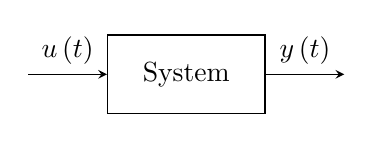
\begin{tikzpicture}[>=stealth]
					\node[draw, rectangle, minimum height=1cm, minimum width=2cm]
					(p) at (0,0) {System};
					\draw[->] ([xshift=-1cm] p.west) -- node[above] {$u\,(t)$} (p.west);
					\draw[->] (p.east) -- node[above] {$y\,(t)$} ([xshift=1cm]p.east);
				\end{tikzpicture}
			\end{center}
		\end{column}
		\pause
		\begin{column}{0.5\textwidth}
			\begin{align*}
				\dot{x}\,(t) & =
				\overbracket{F\,(t)}^{\ast}\,x\,(t) +
				\overbracket{G\,(t)}^{\ast}\,u\,(t) \\
				y\,(t)       & =
				\underbracket{H'(t)}_{\ast}\,x\,(t)
			\end{align*}

			\color{black!60}
			\hspace{0.25cm}$^\ast\,$general model: time-varying;\\
			\hspace{0.25cm}\phantom{$^\ast\,$}if time-invariant often further results
			\color{black}
		\end{column}
	\end{columns}

\end{frame}

% -------------------------------------------------------------------------

\begin{frame}{The regulator problem}

	\begin{columns}
		\begin{column}{0.5\textwidth}

			\begin{block}{Linear Finite-Dimensional}
				\begin{itemize}
					\item $x\,(t) \in \mathbb{R}^n$: system state
					\item $u\,(t) \in \mathbb{R}^m$: system input
					\item $y\,(t) \in \mathbb{R}^p$: system output
				\end{itemize}
			\end{block}

			\begin{center}
				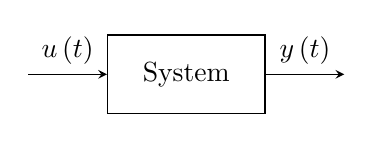
\begin{tikzpicture}[>=stealth]
					\node[draw, rectangle, minimum height=1cm, minimum width=2cm]
					(p) at (0,0) {System};
					\draw[->] ([xshift=-1cm] p.west) -- node[above] {$u\,(t)$} (p.west);
					\draw[->] (p.east) -- node[above] {$y\,(t)$} ([xshift=1cm]p.east);
				\end{tikzpicture}
			\end{center}
		\end{column}
		%
		\begin{column}{0.5\textwidth}
			\begin{align*}
				\dot{x}\,(t) & =
				\overbracket{F\,(t)}^{\ast}\,x\,(t) +
				\overbracket{G\,(t)}^{\ast}\,u\,(t) \\
				y\,(t)       & =
				\underbracket{H'(t)}_{\ast}\,x\,(t)
			\end{align*}

			\color{black!60}
			\hspace{0.25cm}$^\ast\,$general model: time-varying;\\
			\hspace{0.25cm}\phantom{$^\ast\,$}if time-invariant often further results
			\color{black}
		\end{column}
	\end{columns}

	~

	\begin{alertblock}{The regulator problem}
		Suppose that at time $t_0$ some (possibly all) of the values in
		$x\,(t_0)$, $\dot{x}\,(t_0)$, $y\,(t_0)$ are not zero.
		Bring all of them to zero at a finite time $T > t_0$.
	\end{alertblock}

\end{frame}

% -------------------------------------------------------------------------

\begin{frame}{The tracking problem}

	\begin{columns}
		\begin{column}{0.5\textwidth}

			\begin{block}{Linear Finite-Dimensional}
				\begin{itemize}
					\item $x\,(t) \in \mathbb{R}^n$: system state
					\item $u\,(t) \in \mathbb{R}^m$: system input
					\item $y\,(t) \in \mathbb{R}^p$: system output
				\end{itemize}
			\end{block}

			\begin{center}
				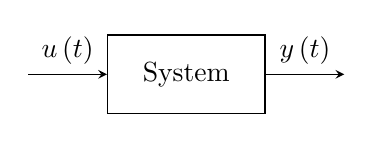
\begin{tikzpicture}[>=stealth]
					\node[draw, rectangle, minimum height=1cm, minimum width=2cm]
					(p) at (0,0) {System};
					\draw[->] ([xshift=-1cm] p.west) -- node[above] {$u\,(t)$} (p.west);
					\draw[->] (p.east) -- node[above] {$y\,(t)$} ([xshift=1cm]p.east);
				\end{tikzpicture}
			\end{center}
		\end{column}
		%
		\begin{column}{0.5\textwidth}
			\begin{align*}
				\dot{x}\,(t) & =
				\overbracket{F\,(t)}^{\ast}\,x\,(t) +
				\overbracket{G\,(t)}^{\ast}\,u\,(t) \\
				y\,(t)       & =
				\underbracket{H'(t)}_{\ast}\,x\,(t)
			\end{align*}

			\color{black!60}
			\hspace{0.25cm}$^\ast\,$general model: time-varying;\\
			\hspace{0.25cm}\phantom{$^\ast\,$}if time-invariant often further results
			\color{black}
		\end{column}
	\end{columns}

	~

	\begin{alertblock}{The tracking problem}
		Given a reference function $\overline{y}\,(t)$ for the output (or for
		the state), make the actual value of $y\,(t)$ follow the reference
		function.
	\end{alertblock}

\end{frame}

% -------------------------------------------------------------------------

\begin{frame}{Example: vehicle control}

	\begin{columns}
		\begin{column}{0.65\textwidth}
			\begin{itemize}
				\item Newton's law: $\overbracket{u\,(t) - \rho(t)\,v\,(t)}^{\text{force}} = \!\!\!\!\!\!\!\! \overbracket{m\,\dot{v}\,(t)}^{\text{mass $\!\cdot\!$ acceleration}}$
				\item Parameters:
				      \begin{itemize}
					      \item[--] $\rho(2.7) = 50\,\text{[N\,s/m]}$: damping coefficient at $2.7$\\
					            (in general, specified as a function of time)
					      \item[--] $m = 1000\,\text[kg]$: vehicle mass (constant)
				      \end{itemize}
				\item Vehicle state: $x_1$ position, $x_2$ velocity
			\end{itemize}

		\end{column}
		\begin{column}{0.35\textwidth}
			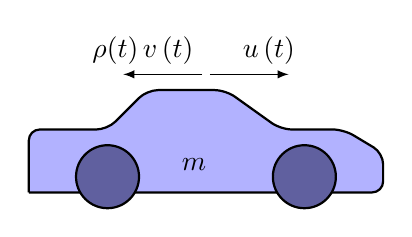
\begin{tikzpicture}

				\draw [thick, fill = blue!30, xshift=-10mm, rounded corners]
				(0,0.2) -- (0,1) -- (1,1) -- (1.5,1.5) -- (2.5,1.5) --
				(3.2,1) -- (4,1) -- (4.5,0.7) -- (4.5,0.2) -- (0,0.2)
				node[midway, xshift=-0.15cm, yshift=0.35cm] {$m$};
				\draw [thick, fill=blue!25!gray] (0mm,4mm) circle (4mm);
				\draw [thick, fill=blue!25!gray] (25mm,4mm) circle (4mm);

				\coordinate (C-G) at (12.5mm,10mm);
				\draw [>=latex,->] (C-G) ++ (-0.05,0.7) -- ++ (-1,0)
				node [near end, sloped, anchor=-90] {$\rho(t)\,v\,(t)$};
				\draw [>=latex,->] (C-G) ++ (0.05,0.7) -- ++ (1,0)
				node [near end, sloped, anchor=-90] {$u\,(t)$};

			\end{tikzpicture}
		\end{column}
	\end{columns}

	~

	\begin{alertblock}{System model}
		$$
			\dot{x}\,(t) =
			\underbracket{\begin{bmatrix} 1 & 0                   \\
                0 & \sfrac{-\rho(t)}{m}\end{bmatrix}}_{F\,(t)} x\,(t) +
			\underbracket{\begin{bmatrix} 0 \\
					\sfrac{1}{m}\end{bmatrix}}_{G} u\,(t);
			\quad\quad
			y\,(t) = \underbracket{\begin{bmatrix} 1 & 0 \\
                0 & 1\end{bmatrix}}_{H^\top = H} x\,(t)
		$$
	\end{alertblock}

\end{frame}

% -------------------------------------------------------------------------

\begin{frame}{Control architecture}

	\begin{columns}
		\begin{column}{0.3\textwidth} \centering
			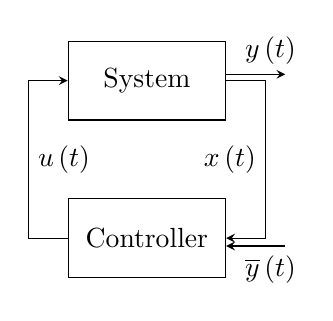
\begin{tikzpicture}[>=stealth]
				\node[draw, rectangle, minimum height=1cm, minimum width=2cm]
				(p) at (0,0) {System};
				\node[draw, rectangle, minimum height=1cm, minimum width=2cm]
				(c) at (0,-2) {Controller};
				\draw[->] (p.east) -- ([xshift=0.5cm]p.east) --
				node[left] {$x\,(t)$}
				([xshift=0.5cm]c.east) -- (c.east);
				\draw[->] (c.west) -- ([xshift=-0.5cm]c.west) --
				node[right] {$u\,(t)$}
				([xshift=-0.5cm]p.west) -- (p.west);
				\draw[->] ([yshift=-0.1cm,xshift=0.75cm]c.east) --
				node[near start,below] {$\overline{y}\,(t)$}
				([yshift=-0.1cm]c.east);
				\draw[<-] ([yshift=0.08cm,xshift=0.75cm]p.east) --
				node[near start,above] {$y\,(t)$}
				([yshift=0.08cm]p.east);
			\end{tikzpicture}\pause

			We start with the regulator problem\vphantom{y}
		\end{column}\pause
		\begin{column}{0.3\textwidth} \centering
			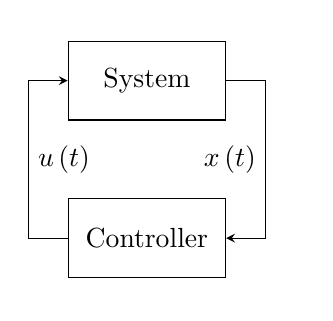
\begin{tikzpicture}[>=stealth]
				\node[draw, rectangle, minimum height=1cm, minimum width=2cm]
				(p) at (0,0) {System};
				\node[draw, rectangle, minimum height=1cm, minimum width=2cm]
				(c) at (0,-2) {Controller};
				\draw[->] (p.east) -- ([xshift=0.5cm]p.east) --
				node[left] {$x\,(t)$}
				([xshift=0.5cm]c.east) -- (c.east);
				\draw[->] (c.west) -- ([xshift=-0.5cm]c.west) --
				node[right] {$u\,(t)$}
				([xshift=-0.5cm]p.west) -- (p.west);
				\phantom{    \draw[->] ([yshift=-0.1cm,xshift=0.75cm]c.east) --
					node[near start,below] {$\overline{y}\,(t)$}
					([yshift=-0.1cm]c.east);}
				\phantom{    \draw[<-] ([yshift=0.08cm,xshift=0.75cm]p.east) --
					node[near start,above] {$y\,(t)$}
					([yshift=0.08cm]p.east);}
			\end{tikzpicture}

			\textcolor{blue}{Assumption}:\\states can be measured\vphantom{y}
		\end{column}\pause
		\begin{column}{0.4\textwidth} \centering
			\begin{tikzpicture}[>=stealth]
				\node[draw=black!50, rectangle, minimum height=1cm, minimum width=2cm]
				(p) at (0,0) {\textcolor{black!50}{System}};
				\node[draw=black!50, rectangle, minimum height=1cm, minimum width=2cm]
				(c) at (0,-2) {\textcolor{black!50}{Controller}};
				\node[draw=black!50, rectangle, minimum height=1cm, minimum width=2cm]
				(e) at (2.5,-1) {\textcolor{black!50}{Estimator}};
				\phantom{    \draw[->] (p.east) -- ([xshift=0.5cm]p.east) --
					node[left] {$x\,(t)$}
					([xshift=0.5cm]c.east) -- (c.east);}
				\draw[->, black!50]
				($([xshift=-0.5cm]c.west)!0.5!([xshift=-0.5cm]p.west)$) --
				(e.west);
				\draw[->, black!50] (c.west) -- ([xshift=-0.5cm]c.west) --
				node[right, fill=white] {$u\,(t)$}
				([xshift=-0.5cm]p.west) -- (p.west);
				\phantom{    \draw[->] ([yshift=-0.1cm,xshift=0.75cm]c.east) --
					node[near start,below] {$\overline{y}\,(t)$}
					([yshift=-0.1cm]c.east);}
				\phantom{    \draw[<-] ([yshift=0.08cm,xshift=0.75cm]p.east) --
					node[near start,above] {$y\,(t)$}
					([yshift=0.08cm]p.east);}
				\draw[->, black!50] (p.east) -| node[above] {$y\,(t)$} (e.north);
				\draw[->, black!50] (e.south) |- node[below] {$\hat{x}\,(t)$} (c.east);
			\end{tikzpicture}

			Future: introducing estimator to relax the \textcolor{blue}{assumption}\vphantom{y}
		\end{column}
	\end{columns}

\end{frame}
